\chapter{Estado del Arte}
\label{sec:EstadoDelArte}

\begin{figure}[htp]
  \centering
  \begin{subfigure}{0.47\textwidth}
    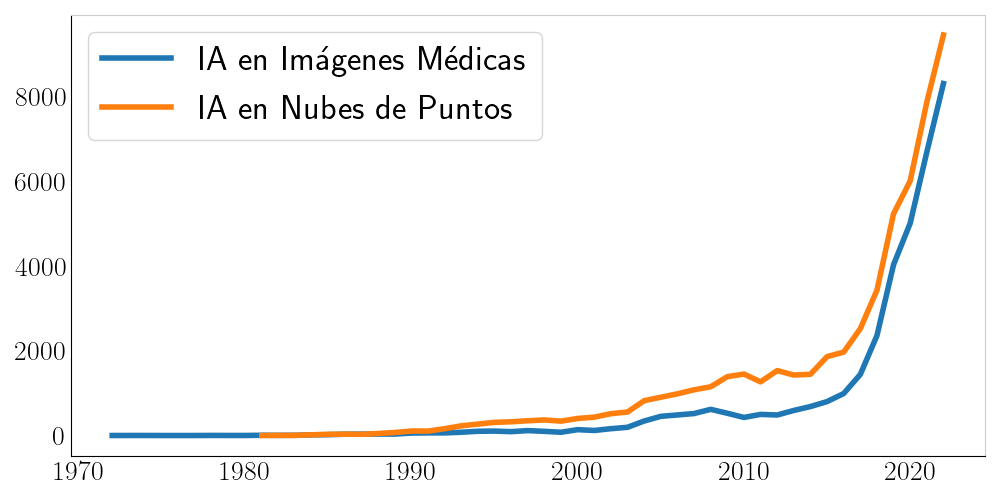
\includegraphics[width=\textwidth]{imagenes/chapter3/ScopusMLinMedicineAndPC.png}
  \end{subfigure}
  \begin{subfigure}{0.47\textwidth}
    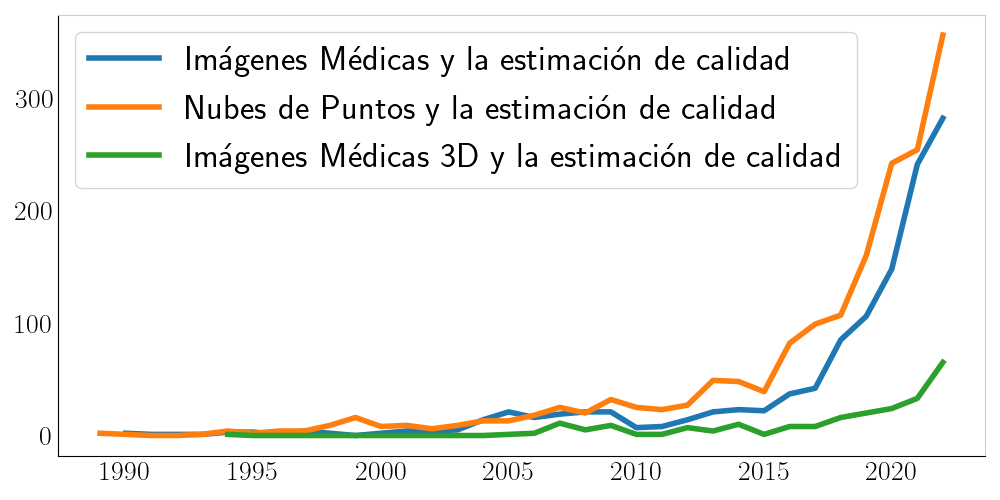
\includegraphics[width=\textwidth]{imagenes/chapter3/ScopusQualityAssessment.png}
  \end{subfigure}
  \caption{Ejemplo de crecimiento de interes en el campo según \emph{Scopus}\footnotemark[1].
  }
  \label{fig:ScopusMLinMedicalAndPC}
\end{figure}
\footnotetext[1]{
Las búsquedas se pueden consultar en el apéndice.
}


\towrite[{Escribir búsquedas en Corpues}]{Hacer introducción y historial de búsqueda de artículos}

Las métricas más populares para la estimación objetiva de la calidad de modelos 
3D basada en puntos son \emph{point-to-point} (Po2Po)\cite{PointToPoint} y
\emph{point-to-plane} (Po2Pl)\cite{PointToPlane}. 
En la primera, para cada punto del objeto distorsionado se obtiene su vecino más cercano en la versión de referencia y 
se calcula alguna métrica de distancia como las discutidas anteriormente (MSE, Minkowski, Hausdorff...). 
La principal desventaja de estos modelos es que no consideran los objetos como 
superficies, aparte de lo comentado en (\ref{fig:FailureMinkowskiMetric},\ref{fig:MSEHyperSphere}).
Para solventar este problema se formuló el segundo método por Tian \emph{et al.} 
que modela la superficie en cada punto como un plano. Ese plano es perpendicular a 
la normal en cada punto. Que se calcula en base a la información de su vencindario. Es decir, 
realizamos los mismos pasos que para la primera, pero proyectamos la distancia sobre 
el vector normal correspondiente. 

Se propuso también otra métrica como \emph{Plane-to-Plane} (Pl2Pl)\cite{PlaneToPlane}, 
que mide la similitud entre superficies associadas a las nubes de puntos. Dentro 
de este mismo ámbito surge también \emph{Point-to-Surface}\cite{PlaneToSurface}, 
que mide la distancia de cada punto de la versión distorsionado respecto a su 
superficie correspondiente en la nube de referencia. Luego para poder tener en
cuenta los colores, surgieron métricas como Po2Po PSNR\cite{PSNR} donde la diferencia 
ya no es respecto a la posición del punto sino que al color en el espacio $YC_bC_r$.

De la información del vecindario de los puntos, gran cantidad de información geométrica 
puede ser extraída para investigar en profundidad la similitud entre las nubes 
de puntos. Surgieron métodos basados en la extracción de características donde la 
mayoría considera tanto información geométrica como los atributos lumínicos.
Existe apenas una métrica que apenas considera características geométricas: PC-MSDM \cite{PC-MSDM}. 
Es una métrica que busca la similitud estructural entre nubes de puntos basándose en
las estadísticas locales de curvatura de los puntos. Esta junto a la información 
extraída de los colores dió lugar a una métrica de similitud de estructuras\cite{PointSSIM}
como adaptación del método \cite{StructuralSimilarityIndex} de IQA a nubes de puntos\cite{SSIM}.  Experimentando con combinaciones de 3 medidas geométricas y 5 comparaciones de color 
para encontrar el mejor vector características resultó en la metrica PCQM\cite{PCQM}.
Similar, utilizando el análisis de componentes principales (PCA) en un vecindario 
de puntos para extraer los valores y vectores singulares por cada punto permitió 
obtener buenos descriptores de información geométrica\cite{PointPCA}.

También se estudió las componentes lumínicas de las nubes de puntos en \cite{ColorBasedObjectiveMetricPC, BitDance}. 
Consistía en generar un histograma y correlograma de la componente lumínica. 
Un correlograma nos permite caracterizar la relación entre pares de variables 
numéricas en un conjunto de datos. Otros, velaron por estudio la energia potencial 
en las nubes de puntos y las diferencias que emergen en presencia de distorsiones\cite{PotentialEnergy}.
Incluso se investigó las transformaciones de datos, se construyeron grafos que representan 
las nubes de puntos, tanto la de referencia como la distorsionada, 
para producir métricas de similitud como GraphSIM y MS-GraphSim\cite{GraphSIM, MS-GraphSim}.

De igual forma, se adaptaron ideas de otros ámbitos, por ejemplo, utilizando 
proyecciones que transladan el mundo tridimensional a un espacio 2D para utilizar 
los métodos más conocidos de estimación de calidad en 2D.
Se realizó incluso un estudio sobre el impacto del número de proyecciones 2D de 
distintas perspectivas en el rendimiento de las métricas de calidad \cite{ImpactOf2DProyections}.

Sin embargo, cuando no tenemos acceso a la nube de puntos de referencia, todas 
estas métricas se ven inutilizables. \emph{Viola et at.}\cite{ViolaRR} propuso 
transferir ciertas características de la nube de punto original antes del proceso
de compresión y transmisión. Con esa información adicional la nube de puntos 
resultantes puede ser evaluada sin la nube de referencia.

\towrite[{Enlazar métodos FR/RR con su casi-similitud a NR}]{Describir similitud en el paso de extracción de características y otros métodos SOTA NR}
